\section{Introduction}
In the previous chapter, a detailed description of the overall autism spectrum disorder
detection process and its various components were presented elaborately. The performance of
the proposed method on the ABIDE dataset will be discussed in this chapter. Our main
objective is to observe how our proposed model performs on unseen data and compute
different performance metrics based on it.\\

This proposed method was implemented in Google Colab notebook using Python language.
The training and testing of the model were carried out using Google Cloud provided backend
free \Gls{TPU} runtime and 12.72 GB RAM on Intel Core i7 processor. It is most unfortunate that
there exists no scope for collecting rs-fMRI scan data from health institutions in Chittagong
due to the unavailability of such modern scan machines. Thus, for conducting this thesis, the
dataset from the open-source multisite ABIDE repository was used.


\section{Dataset Description}
Experimental analysis was conducted over the ABIDE dataset. ABIDE is a consortium that has collected resting-state fMRI data and corresponding phenotypic information of subjects from 17 international sites \cite{di2014autism}. Originally, it contained 1112 scans, including 539 ASD and 573 control individuals. However, all functional data could not pass the QAP (Quality Assessment Protocol) metrics as formulated by the PCP community \cite{abidepreprocessed}, which reduced the size of the dataset to 866 subjects containing 402 ASD and 464 control subjects. Table \ref{tab:4.1} contains the phenotypic information of the participants used in this study.\\

\begin{table}[h!]
\begin{center}
    \caption{Phenotypic information summary of the participants from the ABIDE dataset.}
    \label{tab:4.1}
\begin{tabular}{|l|l|l|l|l|}
\hline
\multicolumn{5}{|c|}{\textbf{Autism Brain Imaging Data Exchange (ABIDE) Dataset}}                                                                                                                                                 \\ \hline
\multicolumn{1}{|c|}{\multirow{2}{*}{\textbf{Site}}} & \multicolumn{3}{c|}{\textbf{Count}}                                                                             & \multicolumn{1}{c|}{\multirow{2}{*}{\textbf{Age Range}}} \\ \cline{2-4}
\multicolumn{1}{|c|}{}                               & \multicolumn{1}{c|}{\textbf{ASD}} & \multicolumn{1}{c|}{\textbf{Control}} & \multicolumn{1}{c|}{\textbf{Total}} & \multicolumn{1}{c|}{}                                    \\ \hline
Caltech                                              & 5                                 & 10                                    & 15                                  & 17–56                                                    \\ \hline
CMU                                                  & 6                                 & 4                                     & 10                                  & 19–40                                                    \\ \hline
KKI                                                  & 12                                & 20                                    & 32                                  & 8–13                                                     \\ \hline
LEUVEN                                               & 26                                & 30                                    & 56                                  & 12–32                                                    \\ \hline
MAX\_MUN                                             & 19                                & 27                                    & 46                                  & 7–58                                                     \\ \hline
NYU                                                  & 74                                & 98                                    & 172                                 & 6–39                                                     \\ \hline
OHSU                                                 & 12                                & 13                                    & 25                                  & 8–15                                                     \\ \hline
OLIN                                                 & 14                                & 14                                    & 28                                  & 10–24                                                    \\ \hline
PITT                                                 & 24                                & 26                                    & 50                                  & 9–35                                                     \\ \hline
SBL                                                  & 12                                & 14                                    & 26                                  & 20–64                                                    \\ \hline
SDSU                                                 & 8                                 & 18                                    & 26                                  & 9–17                                                     \\ \hline
Stanford                                             & 12                                & 13                                    & 25                                  & 8–13                                                     \\ \hline
Trinity                                              & 19                                & 25                                    & 44                                  & 12–26                                                    \\ \hline
UCLA                                                 & 48                                & 37                                    & 85                                  & 8–18                                                     \\ \hline
UM                                                   & 46                                & 73                                    & 119                                 & 8–29                                                     \\ \hline
USM                                                  & 43                                & 24                                    & 67                                  & 9–50                                                     \\ \hline
YALE                                                 & 22                                & 18                                    & 40                                  & 8–18                                                     \\ \hline
TOTAL                                                & 402                               & 464                                   & 866                                 & 6–64                                                     \\ \hline

\end{tabular}
\end{center}
\end{table}

Detailed information about ABIDE dataset is available in \cite{abide}.

\section{Impact Analysis}
The successful implementation of our reasearch work regarding detection of autism spectrum disorder would result in a far-reaching impact in the present diagnosis process. Apart from the applications mentioned previously it would also pose a socio-environmental and ethical impact which are discussed below:

\subsection{Social and Environmental Impact}
The successful implementation of this method may be used for a wide range of applications, such as identifying neural activation patterns responsible for autism and performing visual evaluation of the functional characteristics of the autistic brain. By examining the contrast between the autistic and control brain, the underlying neural or biological basis of ASD can also be unveiled and established. Thus, creating a landmark in the medical diagnostic field.

\subsection{Ethical Impact}
Recent epidemiological investigations have confirmed a dramatic rise in the prevalence of
ASD over the last several decades. Early diagnosis of ASD is indispensable to provide
suitable rehabilitation of the patient at its earliest. It would obstruct the condition from
degrading to a huge extent. But the existing subjective diagnosis process is less available than desired. Many clinics and health institutions do not possess expert clinicians or physicians eligible to conduct these extensive battery of behavioral assessments. Thus, many autistic children are not finally diagnosed until they get older. Such delay in diagnosis can be prevented to a great extent by the introduction of fMRI technique in autism detection. 

\section{Evaluation of Autism Spectrum Disorder Detection Framework}

In this study, preprocessed 4D rs-fMRI data obtained from the ABIDE repository was subsequently converted to 1D feature vector passing through subsequent stages and provided to the deep neural network classifier for generating a prediction. After pre-processing, four different types of brain atlases
were used to extract time-series data from pre-defined ROIs. A sample of time-series data
extracted using BASC atlas comprising 122 ROIs is shown in Figure \ref{fig:4.1}. It has a dimension
of (196, 122) which refers to the average BOLD signal intensity measured from 122 brain
regions at 196 different time-points.

\begin{figure}[h]
\centering
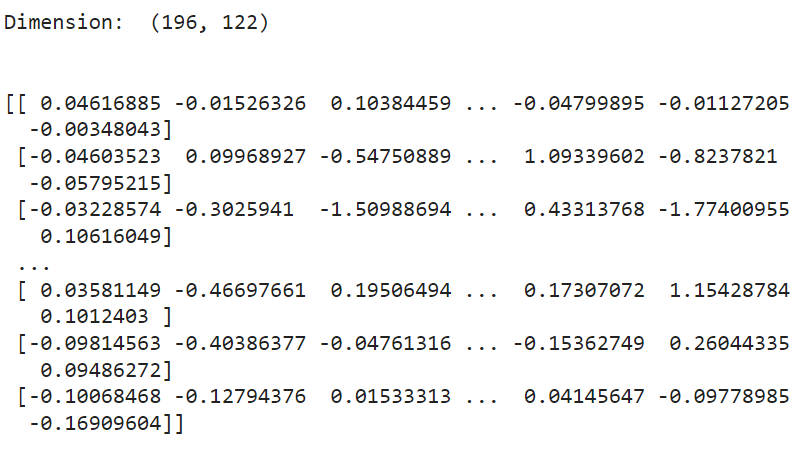
\includegraphics[scale=0.5]{figures/Figure 4.1.png}
\caption{Sample of mean time-series data from a random subject using BASC atlas.}
\label{fig:4.1}
\end{figure}

From the aforementioned time-series data, functional connectivity measures or connectivity
matrices were obtained using tangent space parametrization which converted the (196, 122)
data to a matrix of dimension (122, 122). Finally, the lower half part of this matrix excluding
the diagonal was retrieved and collapsed to form a 1D vector of dimension (7381,) as shown
in Figure \ref{fig:4.2}, since the remaining part of the matrix was redundant. These 1D feature vectors
and corresponding class labels were provided as input to the classifier to get trained on and
perform prediction tasks on the unseen test set.

\begin{figure}[h]
\centering
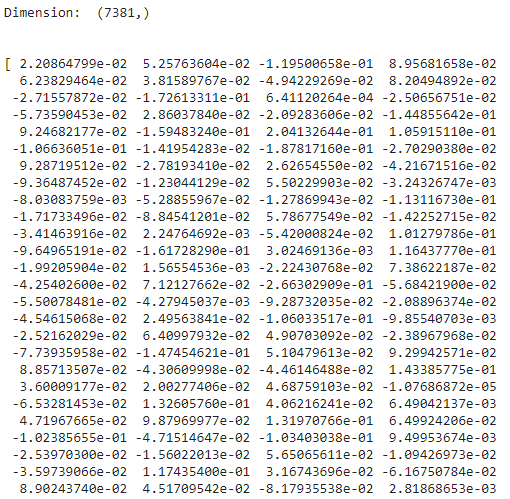
\includegraphics[width=\linewidth]{figures/Figure 4.2.png}
\caption{Sample of feature vector from a random subject using BASC atlas.}
\label{fig:4.2}
\end{figure}

The entire classification task was performed using the Keras API with TensorFlow backend.
For model evaluation, scoring strategy and numerical computation, the scikit learn library
was used. To leverage the power of scikit learn tools while conducting model training and
parameter tuning using Keras API, we used the convenient Keras wrapper function known as
KerasClassifier.The result of the prediction is shown in subsequent sections using a confusion matrix,
different performance measures, plotting the AUC curve, and other performance charts.\\


\section{Evaluation of Performance}
For robust performance evaluation extensive fine-tuning and experimentation were performed in the DNN classifier by varying different hyperparameters. The number of hidden layer neurons of the deep neural network was varied within the range of 8 to 64, and performance was recorded in each case using each of the four atlases. The network structure represented in Figure \ref{fig:3.8}  outperformed other configurations. Each network was validated using the stratified 5-fold cross-validation approach preserving the percentage of subjects in each target class (autism and control) to retain class balance. Twenty percent of the dataset was used as test cases, and the remaining 80\% was utilized in training and validation. Within the training dataset, 80\% of data was used for training and 20\% for validation. A figurative representation of data partitioning is shown in Figure \ref{fig:4.3}. This strategy allowed robust model evaluation while training and testing using different subsets of data.

\begin{figure}[h!]
\centering
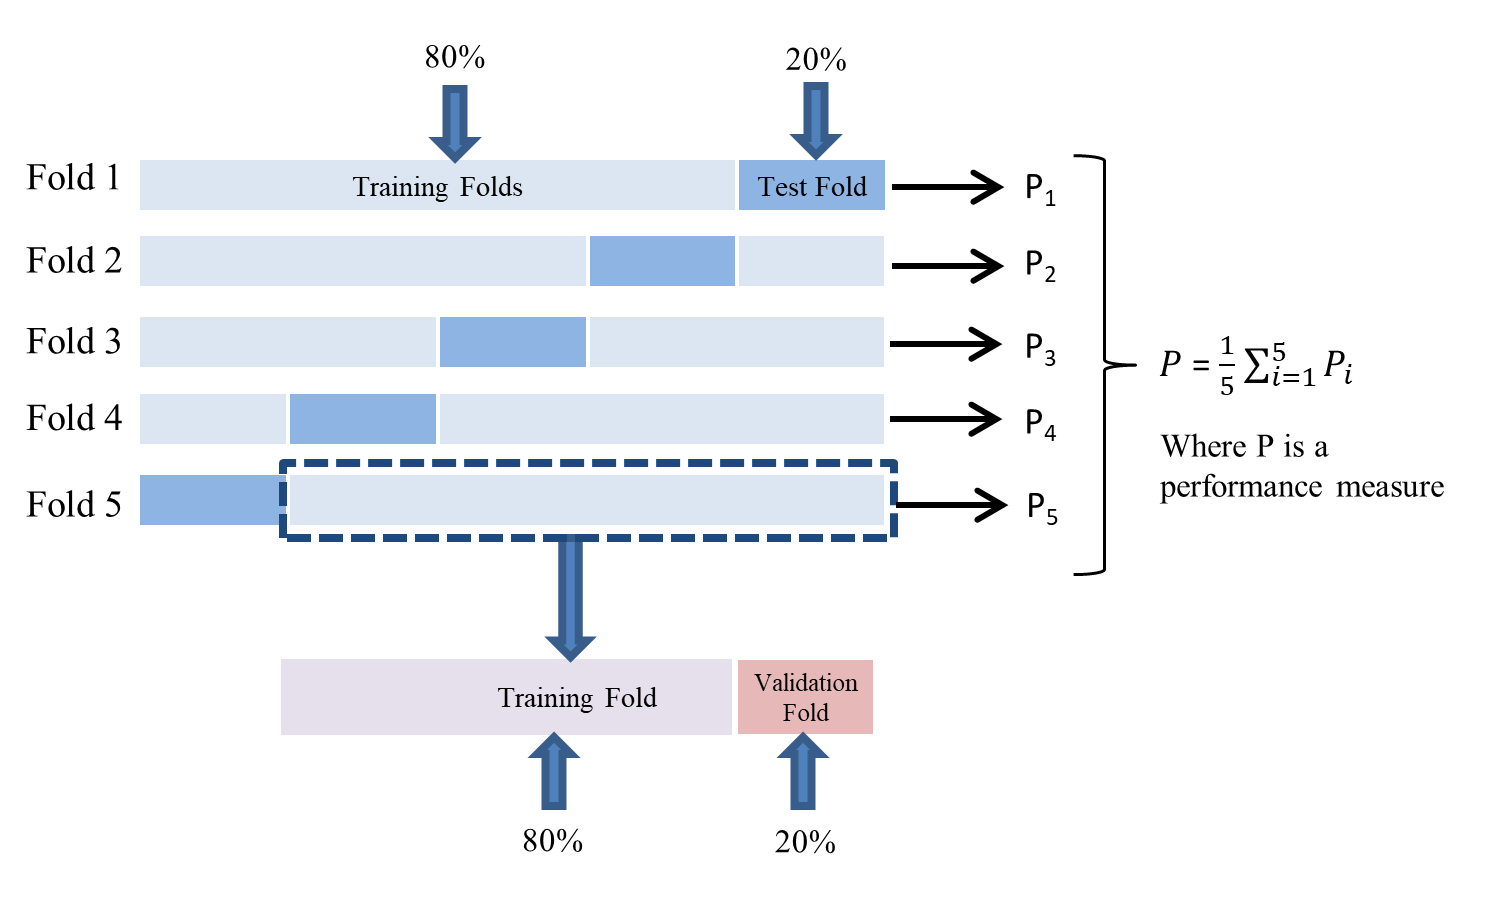
\includegraphics[scale=0.99]{figures/Figure 4.3.png}
\caption{Data partitioning using stratified 5-fold cross-validation.}
\label{fig:4.3}
\end{figure}

Apart from the most commonly used Accuracy metrics, we also measured our model’s
performance using the confusion matrix and other terms associated with it to provide a better
intuition of prediction results.\\

\begin{itemize}
    \item \textbf{Confusion Matrix:} It is a 2x2 matrix for binary classification problems containing
actual labels along one axis and predicted labels along the other axis as depicted in Figure \ref{fig:4.4}

\begin{figure}[h!]
\centering
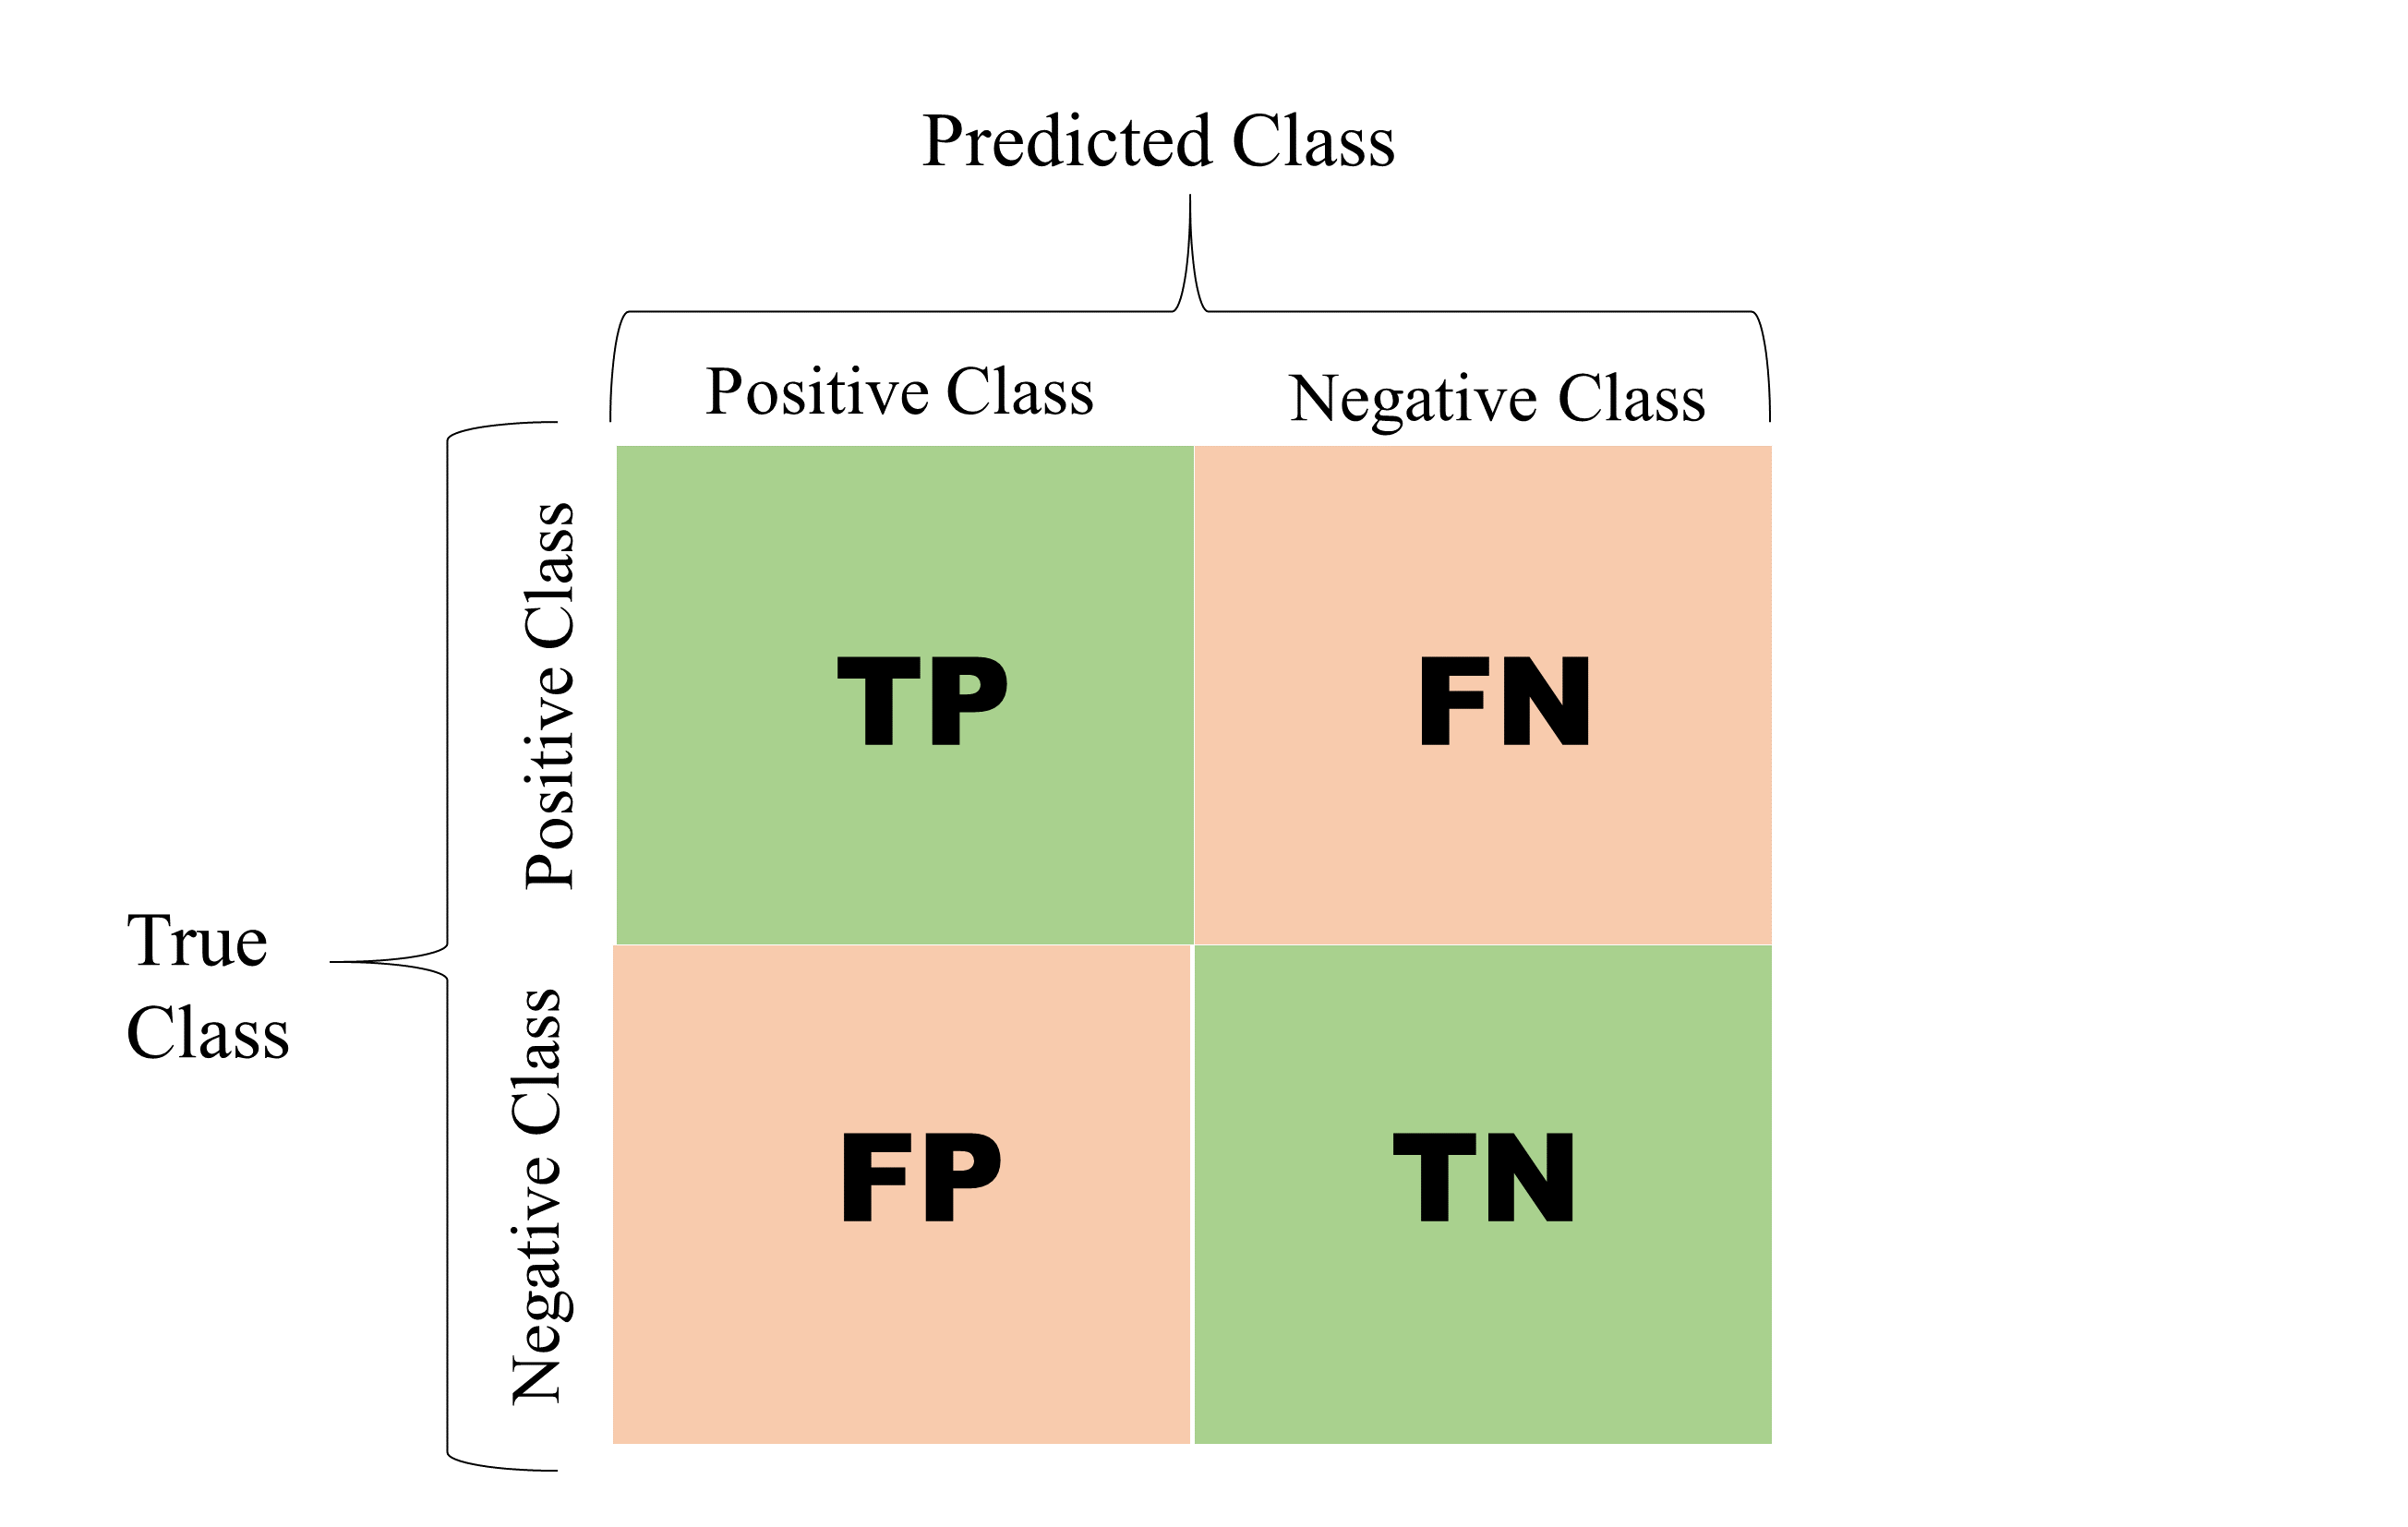
\includegraphics[width=\linewidth]{figures/Figure 4.4.png}
\caption{Confusion Matrix.}
\label{fig:4.4}
\end{figure}

\begin{enumerate}
    \item \textbf{TP:} Positive labels that are correctly classified. In this case, correctly classified autistic
subjects.
\item \textbf{TN:} Negative labels that are correctly classified, i.e, correctly classified control subjects.

\item \textbf{FP:} Actual negative labels that are incorrectly predicted to be positive, i.e, actual
control subjects predicted as autistic subjects.

\item \textbf{FN:} Actual positive labels incorrectly predicted to be negative, i.e, autistic
subjects that are predicted as control.

\end{enumerate}
Using this set of values, the following performance metrics can be derived:


\item $Accuracy=\frac{TP+TN}{TP+TN+FP+FN}$
\item $Precision=\frac{TP}{TP+FP}$
\item $Sensitivity=\frac{TP}{TP+FN}$
\item $Specificity=\frac{TN}{TN+FP}$
\item $F1-Score=\frac{2*Precision*Recall}{Precision+Recall}$
\item \textbf{AUC Curve:} The abbreviation for Area Under ROC (Receiver Operating
Characteristic) Curve. It is a probability curve plotted with TPR (True Positive Rate) against
FPR (False Positive Rate) which serves as a measure of separability between positive and
negative labels. Higher the AUC, better the model in making correct predictions. AUC = 1
represents the best model performance.\\
\end{itemize}

In the following subsections, performance measures using each of the pre-defined atlases
are depicted. Based on the parameters, training data are provided at each fold of the entire
dataset then testing data is supplied for measuring model performance. Finally, an
average performance measure of each metric for all 5 folds are calculated and
represented.

\subsection{Performance Evaluation Using Different Atlas}

Mean performance metrics for different network configurations by fine-tuning using the mentioned atlases are represented in the following subsections. Tables \ref{} represent the value of sensitivity, F1-score, and AUC score for each atlas. Values of mean accuracy and its standard deviation are also shown in percentages. A dropout probability of 0.8 was introduced between each layer to control overfitting, as shown in Figure \ref{fig:3.8}. All the models were compiled using the Adam optimizer with a learning rate of 0.0001 and binary cross-entropy loss function and trained with a batch size of 10. Confusion matrix and mean AUC (area under receiver operating characteristic curve) curves were also represented in each case.

\subsubsection{CC200 Atlas}
Analyzing the mean performance evaluation using five different network configurations from Table \ref{tab:4.2}, it can be observed that CC200 achieved the highest accuracy and F1-score in our proposed Model-2. Though, sensitivity and AUC were the highest for Model-4. However, accuracy and F1 score were relatively lower. Model-2 achieved a relatively good score across all performance metrics. Figure \ref{fig:4.5} represents the confusion matrix and mean AUC curve using the proposed Model-2.

\begin{table}[!htb]
\begin{center}
    \caption{Mean performance evaluation using Craddock 200 (CC200) atlas for different network configurations.}
    \label{tab:4.2}
\begin{tabular}{|l|l|l|l|l|l|l|l|l|}
\hline
\multirow{2}{*}{\textbf{Model}} & \multicolumn{3}{c|}{\textbf{Network Configuration}}                                                                                                                                                       & \multicolumn{5}{c|}{\textbf{\begin{tabular}[c]{@{}c@{}}Mean Performance Evaluation using Craddock 200 \\ (CC200) Atlas\end{tabular}}}                                                                                                       \\ \cline{2-9} 
                                & \textbf{\begin{tabular}[c]{@{}l@{}}Input \\ Layer\end{tabular}} & \textbf{\begin{tabular}[c]{@{}l@{}}Hidden \\ Layer 1\end{tabular}} & \textbf{\begin{tabular}[c]{@{}l@{}}Hidden \\ Layer 2\end{tabular}} & \textbf{Accuracy} & \textbf{\begin{tabular}[c]{@{}l@{}}Acc.Std  \\ (\%)\end{tabular}} & \textbf{Sensitivity} & \textbf{\begin{tabular}[c]{@{}l@{}}F1-\\ Score\end{tabular}} & \textbf{\begin{tabular}[c]{@{}l@{}}AUC \\ Score\end{tabular}} \\ \hline
Model-1                         & 19900                                                           & 64                                                                 & 32                                                                 & 0.8473            & 1.57                                                              & 0.9406               & 0.8510                                                       & 0.9515                                                        \\ \hline
\textbf{Model-2}                & \textbf{19900}                                                  & \textbf{32}                                                        & \textbf{32}                                                        & \textbf{0.8668}   & \textbf{2.38}                                                     & \textbf{0.8683}      & \textbf{0.8579}                                              & \textbf{0.9571}                                               \\ \hline
Model-3                         & 19900                                                           & 32                                                                 & 16                                                                 & 0.8530            & 3.02                                                              & 0.7194               & 0.8185                                                       & 0.9569                                                        \\ \hline
Model-4                         & 19900                                                           & 16                                                                 & 16                                                                 & 0.6843            & 2.74                                                              & 0.9429               & 0.7343                                                       & 0.9595                                                        \\ \hline
Model-5                         & 19900                                                           & 16                                                                 & 8                                                                  & 0.5947            & 4.23                                                              & 0.9182               & 0.6770                                                       & 0.9592                                                        \\ \hline
\end{tabular}
\end{center}
\end{table}

\begin{figure}[h!]
\centering
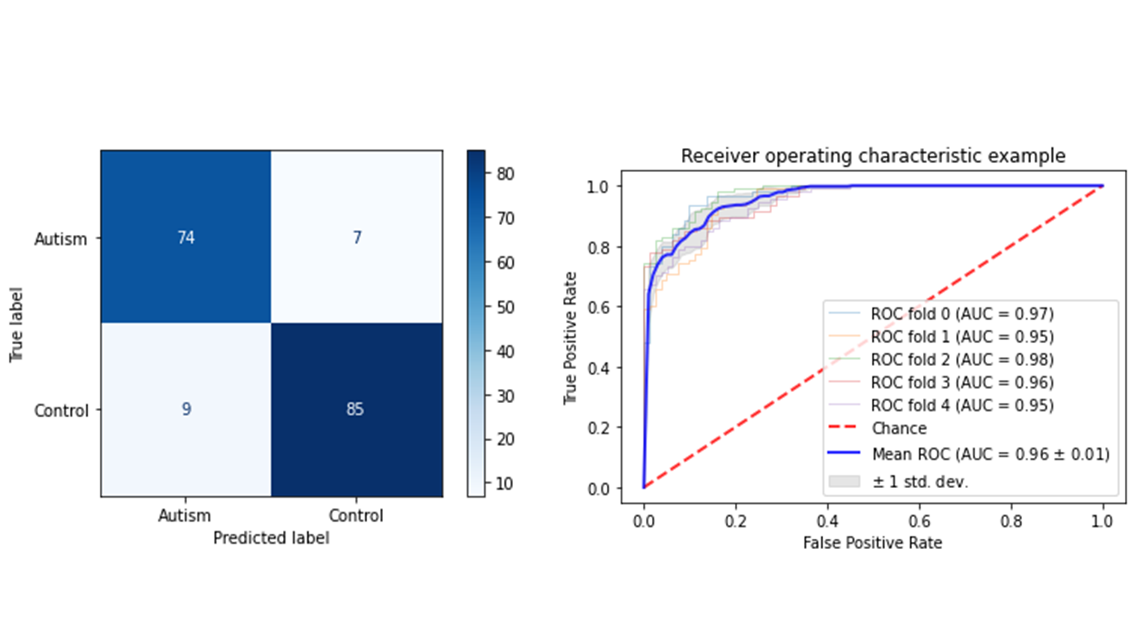
\includegraphics[width=\linewidth]{figures/Figure 4.5.png}
\caption{Confusion matrix and area under receiver operator characteristic curve (AUC) curve for CC200 atlas using Model-2.}
\label{fig:4.5}
\end{figure}

\subsubsection{Power Atlas}
From Table \ref{tab:4.3}, it is observed that the proposed Model-2 achieved a superior F1-score while the remaining scores were also greater than 85\%. Model-5 obtained the highest sensitivity while accuracy and F1-score remained poor. AUC score remained almost constant at 95\% for all models. Figure \ref{fig:4.6} represents the confusion matrix and mean AUC curve using the proposed Model-2.

\begin{table}[!htb]
\begin{center}
    \caption{Mean performance evaluation using Power atlas for different network configurations.}
    \label{tab:4.3}
\begin{tabular}{|l|l|l|l|l|l|l|l|l|}
\hline
\multirow{2}{*}{\textbf{Model}} & \multicolumn{3}{c|}{\textbf{Network Configuration}}                                                                                                                                                       & \multicolumn{5}{c|}{\textbf{\begin{tabular}[c]{@{}c@{}}Mean Performance Evaluation using \\ Power Atlas\end{tabular}}}                                                                                                                      \\ \cline{2-9} 
                                & \textbf{\begin{tabular}[c]{@{}l@{}}Input \\ Layer\end{tabular}} & \textbf{\begin{tabular}[c]{@{}l@{}}Hidden \\ Layer 1\end{tabular}} & \textbf{\begin{tabular}[c]{@{}l@{}}Hidden \\ Layer 2\end{tabular}} & \textbf{Accuracy} & \textbf{\begin{tabular}[c]{@{}l@{}}Acc.Std  \\ (\%)\end{tabular}} & \textbf{Sensitivity} & \textbf{\begin{tabular}[c]{@{}l@{}}F1-\\ Score\end{tabular}} & \textbf{\begin{tabular}[c]{@{}l@{}}AUC \\ Score\end{tabular}} \\ \hline
Model-1                         & 34716                                                           & 64                                                                 & 32                                                                 & 0.7898            & 2.12                                                              & 0.9626               & 0.8098                                                       & 0.9513                                                        \\ \hline
\textbf{Model-2}                & \textbf{34716}                                                  & \textbf{32}                                                        & \textbf{32}                                                        & \textbf{0.8533}   & \textbf{2.38}                                                     & \textbf{0.8633}      & \textbf{0.8453}                                              & \textbf{0.9531}                                               \\ \hline
Model-3                         & 34716                                                           & 32                                                                 & 16                                                                 & 0.8245            & 2.31                                                              & 0.9429               & 0.8335                                                       & 0.9505                                                        \\ \hline
Model-4                         & 34716                                                           & 16                                                                 & 16                                                                 & 0.8638            & 3.22                                                              & 0.7662               & 0.8385                                                       & 0.9565                                                        \\ \hline
Model-5                         & 34716                                                           & 16                                                                 & 8                                                                  & 0.5993            & 2.16                                                              & 0.9802               & 0.6946                                                       & 0.9509                                                        \\ \hline
\end{tabular}
\end{center}
\end{table}

\begin{figure}[h!]
\centering
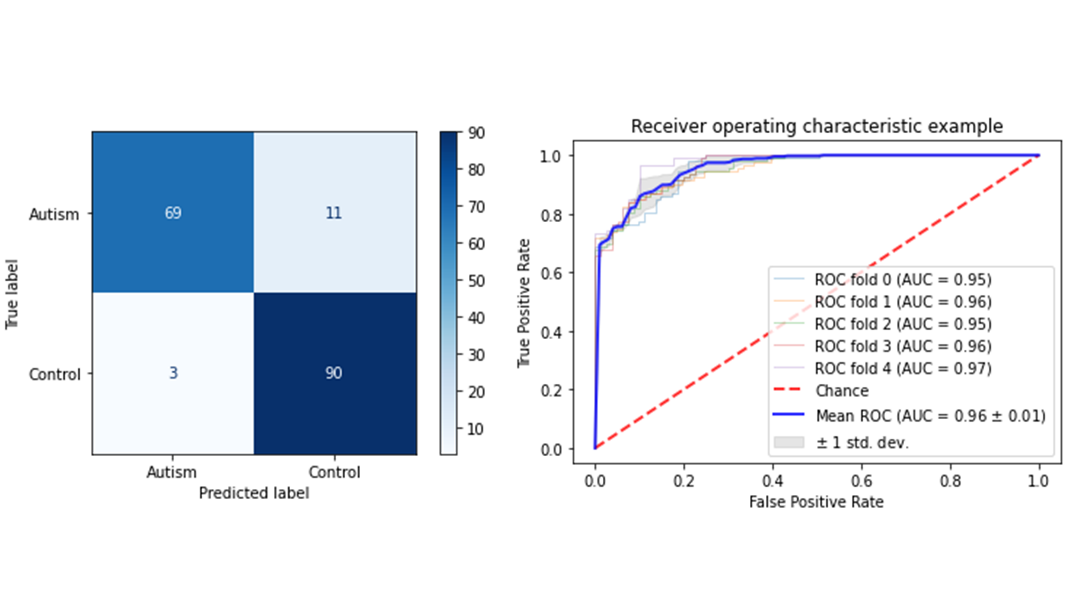
\includegraphics[width=\linewidth]{figures/Figure 4.6.png}
\caption{Confusion matrix and area under receiver operator characteristic curve (AUC) curve for Power atlas using Model-2.}
\label{fig:4.6}
\end{figure}

\subsubsection{BASC Atlas}

Table \ref{tab:4.4} shows that the BASC atlas achieved the highest performance measure across all performance metrics using the proposed model. Figure \ref{fig:4.7} contains the confusion matrix and AUC curve using Model-2.

\begin{table}[!htb]
\begin{center}
    \caption{Mean performance evaluation using BASC atlas for different network configurations.}
    \label{tab:4.4}
\begin{tabular}{|l|l|l|l|l|l|l|l|l|}
\hline
\multirow{2}{*}{\textbf{Model}} & \multicolumn{3}{c|}{\textbf{Network Configuration}}                                                                                                                                                       & \multicolumn{5}{c|}{\textbf{\begin{tabular}[c]{@{}c@{}}Mean Performance Evaluation using \\ Bootstrap Analysis of Stable Clusters (BASC) atlas\end{tabular}}}                                                                               \\ \cline{2-9} 
                                & \textbf{\begin{tabular}[c]{@{}l@{}}Input \\ Layer\end{tabular}} & \textbf{\begin{tabular}[c]{@{}l@{}}Hidden \\ Layer 1\end{tabular}} & \textbf{\begin{tabular}[c]{@{}l@{}}Hidden \\ Layer 2\end{tabular}} & \textbf{Accuracy} & \textbf{\begin{tabular}[c]{@{}l@{}}Acc.Std  \\ (\%)\end{tabular}} & \textbf{Sensitivity} & \textbf{\begin{tabular}[c]{@{}l@{}}F1-\\ Score\end{tabular}} & \textbf{\begin{tabular}[c]{@{}l@{}}AUC \\ Score\end{tabular}} \\ \hline
Model-1                         & 7381                                                            & 64                                                                 & 32                                                                 & 0.8557            & 2.76                                                              & 0.8634               & 0.8467                                                       & 0.9570                                                        \\ \hline
\textbf{Model-2}                & \textbf{7381}                                                   & \textbf{32}                                                        & \textbf{32}                                                        & \textbf{0.8787}   & \textbf{2.33}                                                     & \textbf{0.9029}      & \textbf{0.8739}                                              & \textbf{0.9587}                                               \\ \hline
Model-3                         & 7381                                                            & 32                                                                 & 16                                                                 & 0.8672            & 2.49                                                              & 0.8507               & 0.8563                                                       & 0.9439                                                        \\ \hline
Model-4                         & 7381                                                            & 16                                                                 & 16                                                                 & 0.8545            & 2.51                                                              & 0.8358               & 0.8419                                                       & 0.9471                                                        \\ \hline
Model-5                         & 7381                                                            & 16                                                                 & 8                                                                  & 0.8579            & 1.90                                                              & 0.8731               & 0.8511                                                       & 0.9418                                                        \\ \hline
\end{tabular}
\end{center}
\end{table}

\begin{figure}[h!]
\centering
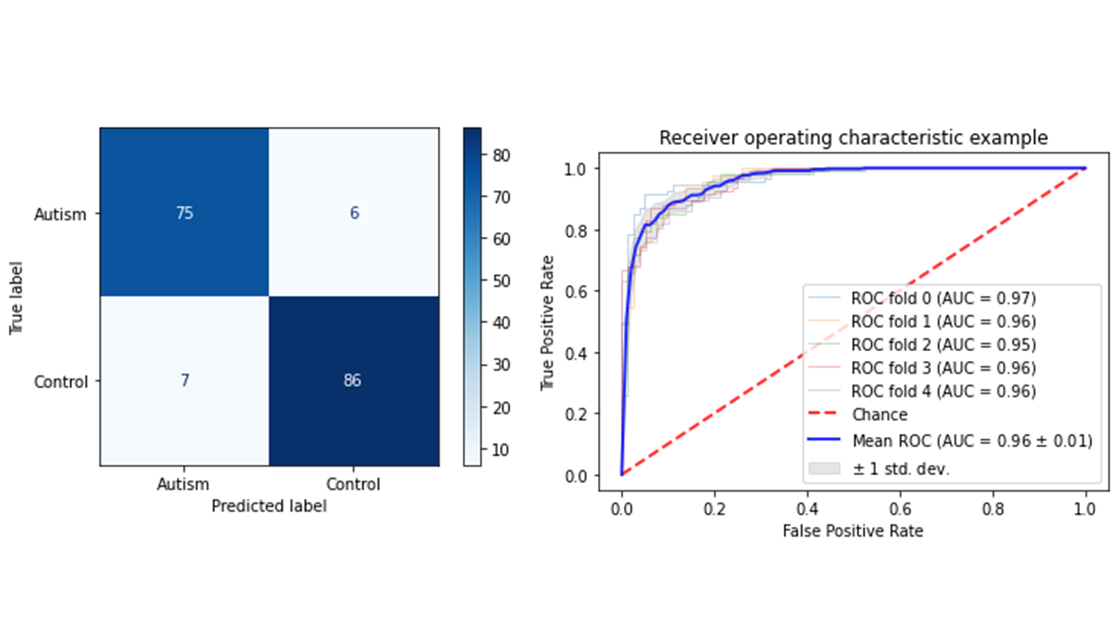
\includegraphics[width=\linewidth]{figures/Figure 4.7.png}
\caption{Confusion matrix and area under receiver operator characteristic curve (AUC) curve for BASC atlas using Model-2.}
\label{fig:4.7}
\end{figure}

\subsubsection{AAL Atlas}

From Table \ref{tab:4.5}, it is evident that AAL atlas represented a fluctuating performance across different models for each scoring metric. The confusion matrix and AUC curve using Model-2 are illustrated in Figure \ref{fig:4.8}.

\begin{table}[!htb]
\begin{center}
    \caption{Mean performance evaluation using AAL atlas for different network configurations.}
    \label{tab:4.5}
\begin{tabular}{|l|l|l|l|l|l|l|l|l|}
\hline
\multirow{2}{*}{\textbf{Model}} & \multicolumn{3}{c|}{\textbf{Network Configuration}}                                                                                                                                                       & \multicolumn{5}{c|}{\textbf{\begin{tabular}[c]{@{}c@{}}Mean Performance Evaluation using \\ Automated Anatomical Labeling (AAL) atlas\end{tabular}}}                                                                                        \\ \cline{2-9} 
                                & \textbf{\begin{tabular}[c]{@{}l@{}}Input \\ Layer\end{tabular}} & \textbf{\begin{tabular}[c]{@{}l@{}}Hidden \\ Layer 1\end{tabular}} & \textbf{\begin{tabular}[c]{@{}l@{}}Hidden \\ Layer 2\end{tabular}} & \textbf{Accuracy} & \textbf{\begin{tabular}[c]{@{}l@{}}Acc.Std  \\ (\%)\end{tabular}} & \textbf{Sensitivity} & \textbf{\begin{tabular}[c]{@{}l@{}}F1-\\ Score\end{tabular}} & \textbf{\begin{tabular}[c]{@{}l@{}}AUC \\ Score\end{tabular}} \\ \hline
Model-1                         & 6670                                                            & 64                                                                 & 32                                                                 & 0.8611            & 2.59                                                              & 0.8933               & 0.8561                                                       & 0.9523                                                        \\ \hline
\textbf{Model-2}                & \textbf{6670}                                                   & \textbf{32}                                                        & \textbf{32}                                                        & \textbf{0.8737}   & \textbf{2.49}                                                     & \textbf{0.8412}      & \textbf{0.8599}                                              & \textbf{0.9512}                                               \\ \hline
Model-3                         & 6670                                                            & 32                                                                 & 16                                                                 & 0.8679            & 3.77                                                              & 0.7941               & 0.8475                                                       & 0.9500                                                        \\ \hline
Model-4                         & 6670                                                            & 16                                                                 & 16                                                                 & 0.8702            & 3.95                                                              & 0.9082               & 0.8665                                                       & 0.9522                                                        \\ \hline
Model-5                         & 6670                                                            & 16                                                                 & 8                                                                  & 0.8312            & 2.73                                                              & 0.9404               & 0.8379                                                       & 0.9509                                                        \\ \hline
\end{tabular}
\end{center}
\end{table}

\begin{figure}[h!]
\centering
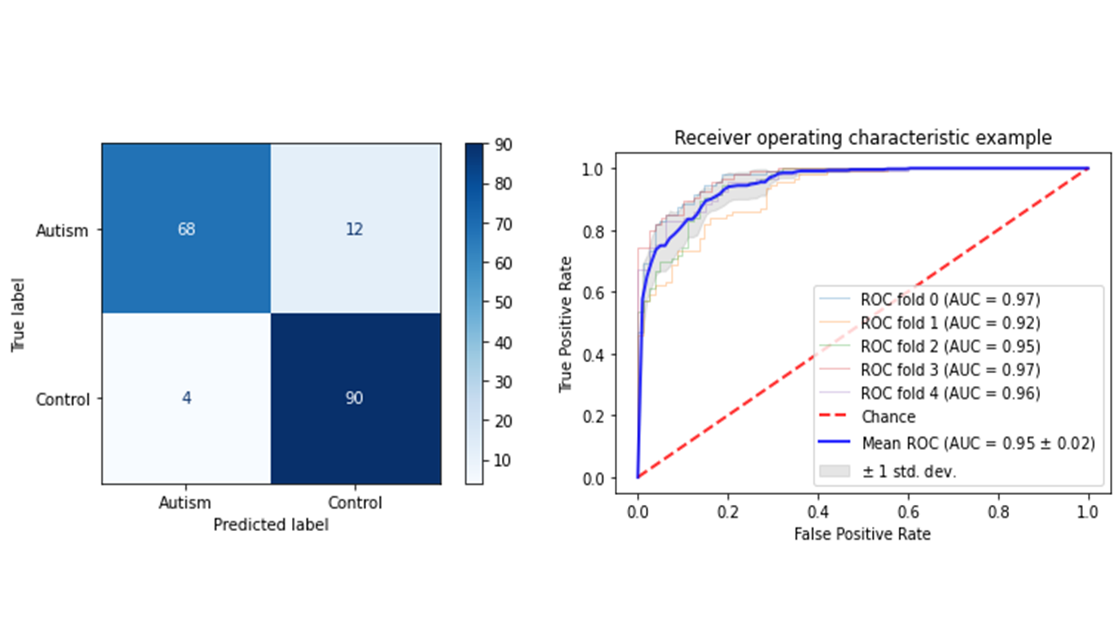
\includegraphics[width=\linewidth]{figures/Figure 4.8.png}
\caption{Confusion matrix and area under receiver operator characteristic curve (AUC) curve for AAL atlas using Model-2.}
\label{fig:4.5}
\end{figure}

\subsection{Performance Comparison among Atlases}
A comparison of all performance metrics across all four atlases is represented in Figure \ref{fig:4.9} using the proposed Model-2 to determine which atlas had the most discriminative power in identifying autism and control cases.

\begin{figure}[h!]
\centering
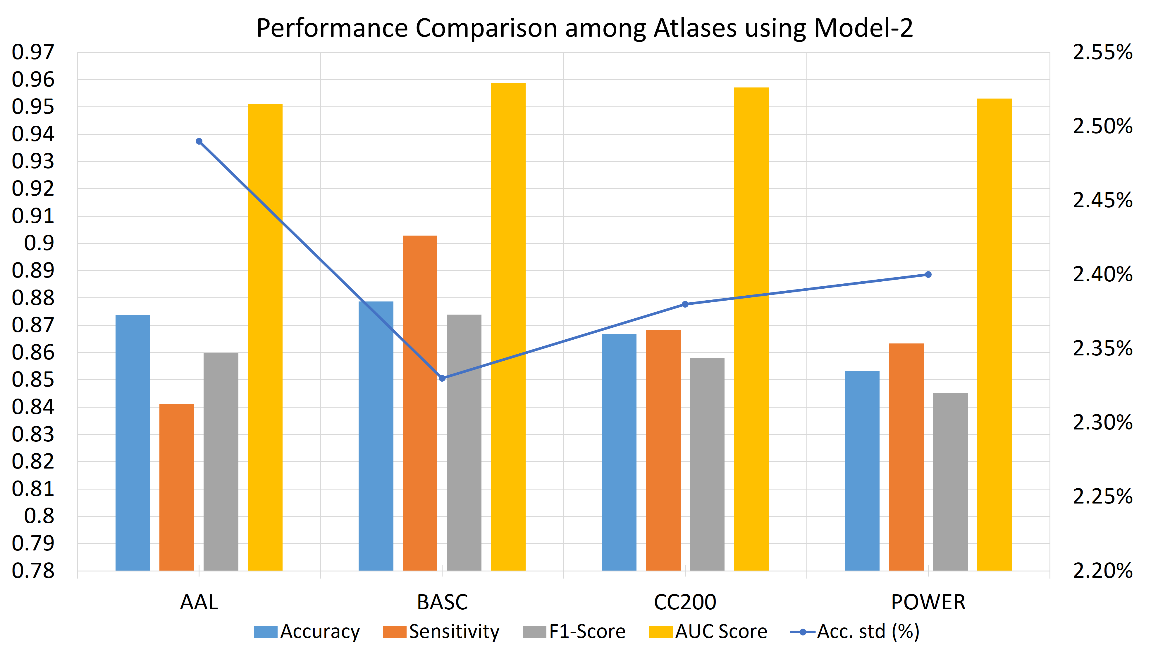
\includegraphics[width=\linewidth]{figures/Figure 4.9.png}
\caption{Performance comparison among atlases using Model-2.}
\label{fig:4.9}
\end{figure}

From the above graphical analysis, the following points can be demonstrated:\\

\begin{itemize}
    \item BASC atlas provided superior performance in terms of accuracy, sensitivity, F1, and AUC score using the proposed Model-2.
    \item AAL showed inconsistent results among various metrics. It had the lowest sensitivity value, which is very crucial and significant in medical diagnosis.
    \item CC200 and Power atlas depicted the lowest predictive power based on its performance value across all measures.
    \item The blue line chart depicts the standard deviation in percentage in terms of accuracy. BASC atlas has the least amount of deviation while AAL has maximum deviation.
\end{itemize}

From the aforementioned points, it can be concluded that the BASC atlas displays the best performance across all metrics. It exhibits the highest discriminative power in a balanced manner which is evident from its F1 score. Other models exceeding two hidden layers were also attempted, but experimental results deteriorated due to the limited dataset.

\subsection{Performance Comparison Using BASC Atlas and Single-Site Data}

A quantitative analysis of accuracy, sensitivity, and F1-score obtained by testing the proposed Model-2 classifier on data obtained from individual screening sites of ABIDE is represented in Table \ref{tab:4.6} using BASC atlas.

\begin{table}[!htb]
\begin{center}
    \caption{Performance comparison using Model-2 and BASC atlas on data obtained from 
individual screening sites.}
    \label{tab:4.6}
\begin{tabular}{|l|l|l|l|l|}
\hline
\textbf{Site ID} & \textbf{No of Subjects} & \textbf{Accuracy} & \textbf{Sensitivity} & \textbf{F1-Score} \\ \hline
PITT             & 50                      & 0.94              & 0.96                 & 0.94              \\ \hline
YALE             & 40                      & 0.95              & 0.91                 & 0.95              \\ \hline
NYU              & 172                     & 0.92              & 0.92                 & 0.91              \\ \hline
UM               & 119                     & 0.93              & 0.92                 & 0.92              \\ \hline
\end{tabular}
\end{center}
\end{table}

From the above tabular analysis, a significant improvement in performance can be observed across different performance metrics while using data obtained from individual screening sites. On the contrary, performance drops when the entire ABIDE dataset comprising 17 international sites was used for testing. This is because different sites use different MRI acquisition protocols, scanning parameters, ways of laying the participants in the scanner, etc., which introduces huge variance across datasets obtained from different sites. Moreover, the effect of domain shift and distributional shift might also be responsible for such differences in performance measures.

\subsection{Performance Comparison with Machine Learning\\ Methods}
Performance of machine learning classifiers, such as k-nearest neighbors (KNN), Random Forest, Naïve Bayes, etc., to successfully predict functional connectivity-based classification have been compared across rs-fMRI cohorts by Dadi et al. in \cite{dadi2019benchmarking}. To our knowledge, no such comparative analysis has been conducted using deep learning classifiers as of now. In Figure \ref{fig:4.10}, a performance comparison between popular machine learning algorithms and our proposed Model-2 is represented. From this table, it is evident that our proposed deep learning model outperformed the machine learning techniques.


\begin{figure}[h!]
\centering
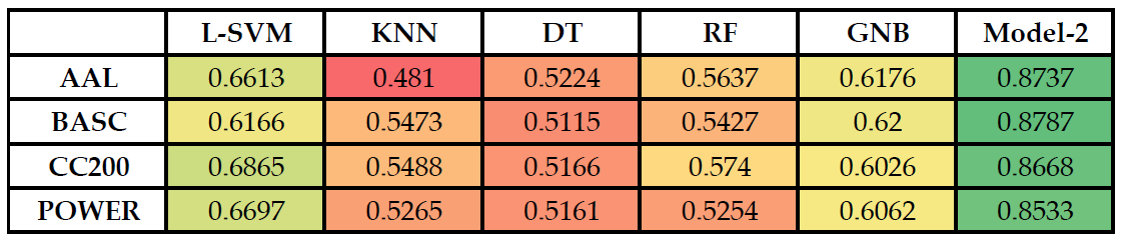
\includegraphics[width=\textwidth]{figures/Figure 4.10.png}
\caption{Performance comparison with different machine learning algorithms.}
\label{fig:4.10}
\end{figure}

Here, L-SVM indicates linear support vector machine; KNN means k-nearest neighbor; DT represents decision tree; RF indicates random forest and GNB means Gaussian Naïve Bayes classifier. Performance was measured using accuracy metrics. The Green–Yellow–Red color scale is used to highlight the performances where green indicates superior performance and red indicates the lowest performance.

\subsection{Performance Comparison with Existing Literature}

Table \ref{tab:4.7} illustrates the highest performance measure obtained from different existing works related to fMRI based ASD identification using brain atlases and our proposed model.

\begin{table}[!htb]
\begin{center}
    \caption{Performance comparison with existing literature.}
    \label{tab:4.7}
\begin{tabular}{|l|l|l|}
\hline
\textbf{Methods}          & \textbf{Year   Published} & \textbf{Accuracy   (\%)} \\ \hline
Heinsfeld et al. \cite{heinsfeld2018identification} & 2018                      & 70.00                    \\ \hline
Eslami et al. \cite{eslami2019asd}    & 2019                      & 70.30                    \\ \hline
Wang et al. \cite{wang2020aimafe}      & 2020                      & 74.52                    \\ \hline
Yang et al. \cite{yangdeep}      & 2020                      & 75.27                    \\ \hline
Tang et al. \cite{tang2020deep}     & 2020                      & 74.00                    \\ \hline
Our Proposed Model. \cite{subah2021deep}        & 2021                        & 87.87                    \\ \hline
\end{tabular}
\end{center}
\end{table}

From above analysis it can be stated that the present study marked a significant performance improvement compared to existing studies.  
In our study, all the features extracted from the ROIs defined by each brain atlases were
provided to the DNN classifier. Regardless of the size of the feature vector obtained after flattening of the functional connectivity matrix, no feature selection technique was used to select notable features while discarding the
rest to reduce the risk of overfitting due to high dimensionality. In fact, dropout layers were introduced between each hidden layers to prevent
overfitting. As such, all the features obtained from ROIs defined by the atlases (no
matter how minimal or tremendous its effect might be in discriminating the two
groups of participants) contributed to the ASD classification task which might be the
reason for obtaining such an optimistic result. Besides, the use of
suitable optimizer, weight initialization technique, learning rate, dropout rate, etc by
fine-tuning also helps the neural network to extract meaningful information from the
provided features that increases prediction accuracy compared to other 
methods that involved featured selection techniques. 

\section{Conclusion}
This chapter provides the results of our proposed ASD detection framework and performs
performance evaluation in multifarious ways. The comparative performances across different
brain atlases, traditional machine learning methods and existing studies are also represented
here. From all these perspective, our proposed framework using BASC atlas comprising 122
ROIs proved to be superior. The next chapter concludes this thesis and provides future
recommendations.